\documentclass[presentation.tex]{subfiles} 

\begin{document}	
	\begin{frame}
		\frametitle{Implementácia}
		\begin{itemize}
			\item upravený tvar úlohy pre solver
		\end{itemize}
		\begin{align*}
			\text{min}~ &c^Tx\\
			&A_{ub}x \leq b_{ub} \\
			&A_{eq}x = b_{eq} \\
			&x \in [l, u] & l \leq u;~l,u \in (\mathbb{R}\cup \{-\infty, \infty\})^n 
		\end{align*}
	\end{frame}
	
	
	\begin{frame}[fragile]
		\frametitle{Implementácia}
		\begin{python}
c = np.concatenate(([0]*(k + 1), np.ones(n))) 
A = np.block([np.ones((n, 1)), np.array(x.values)])
I = np.identity(n)

A_ub = np.block([[-A, -I], [A, -I]])
b_ub = np.concatenate([-y, y])
bounds = [(None, None)]*(k + 1) + [(0, None)] * n
		\end{python}
	\end{frame}
	
	\begin{frame}[fragile]
		\frametitle{Riešenie úlohy a vizualizácia}
		\begin{columns}
		\begin{column}{0.6\textwidth}
			\begin{python}
solve = linprog(c, A_ub, b_ub, bounds=bounds)
betas = solve.x[:k+1]
			\end{python}
		\end{column}
		\begin{column}{0.4\textwidth}
			\captionsetup{justification=centering}
			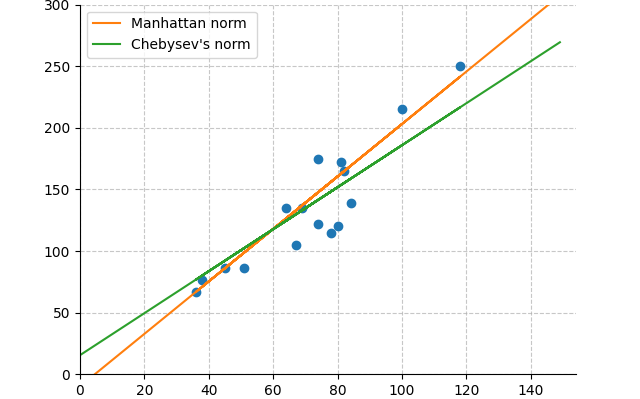
\includegraphics[width=1\linewidth]{../report/figs/task_b_plot-cropped.png}
			\captionof*{figure}{priamky $L^1$ a $L^{\infty}$ lineárnych regresií pre arbitrárne dáta}
		\end{column}
		\end{columns}

	\end{frame}
	
\end{document}